\documentclass{standalone}
\usepackage{tikz}
\usetikzlibrary{patterns}
\usetikzlibrary{positioning}
\usetikzlibrary{patterns, positioning}
\usetikzlibrary{shapes.misc}
\usepackage[outline]{contour}
\contourlength{1.5pt} 
\usetikzlibrary{calc}
        \usepackage{relsize}
        \tikzset{fontscale/.style = {font=\relsize{#1}}}

\begin{document}
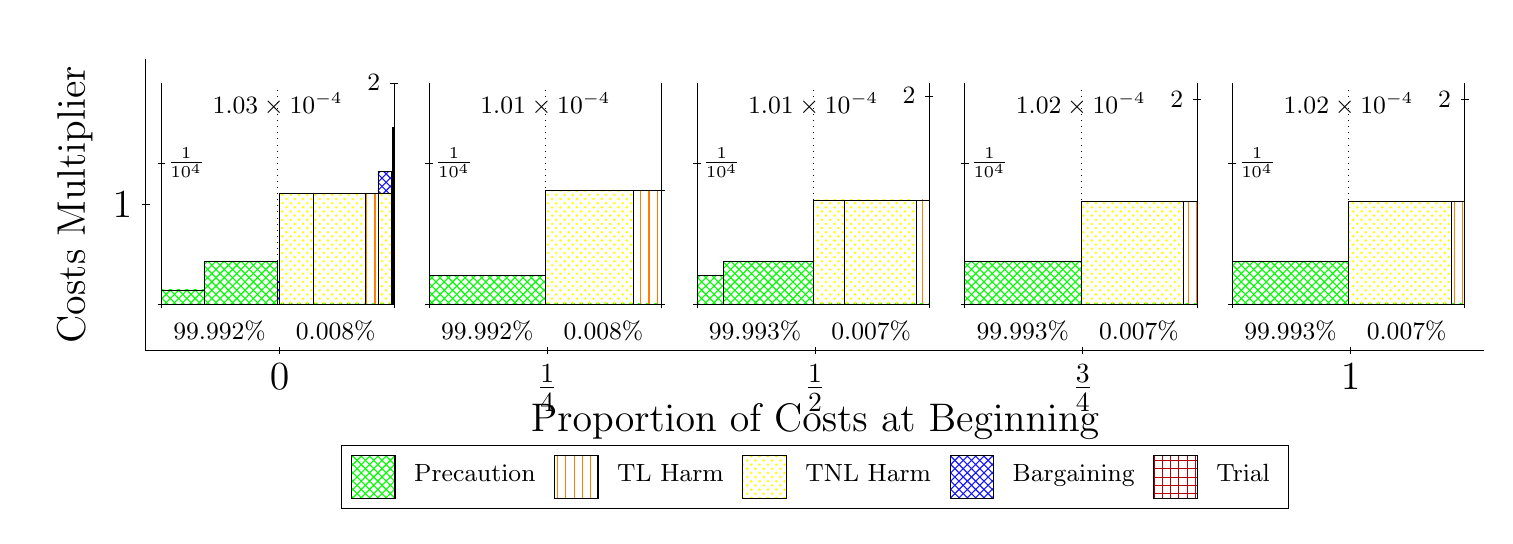
\begin{tikzpicture}
\clip(-0.5,-1.1) rectangle +(18.5,6.2);
\draw[black] (1,1) -- (1,4.7);
\node[rotate=90, fontscale=2, anchor=center] at (0.1, 2.85) {Costs Multiplier};
\draw[black] (0.95,2.85) -- (1.05,2.85);
\node[fontscale=2, anchor=east] at (0.95, 2.85) {1};

\draw[black] (1,1) -- (18,1);
\node[fontscale=2, anchor=center] at (9.5, 0.1) {Proportion of Costs at Beginning};
\draw[black] (2.7,0.95) -- (2.7,1.05);
\node[fontscale=2, anchor=north] at (2.7, 0.95) {0};
\draw[black] (6.1,0.95) -- (6.1,1.05);
\node[fontscale=2, anchor=north] at (6.1, 0.95) {$\frac{1}{4}$};
\draw[black] (9.5,0.95) -- (9.5,1.05);
\node[fontscale=2, anchor=north] at (9.5, 0.95) {$\frac{1}{2}$};
\draw[black] (12.9,0.95) -- (12.9,1.05);
\node[fontscale=2, anchor=north] at (12.9, 0.95) {$\frac{3}{4}$};
\draw[black] (16.3,0.95) -- (16.3,1.05);
\node[fontscale=2, anchor=north] at (16.3, 0.95) {1};


\draw[pattern=crosshatch, pattern color=green,draw=black,very thin] (1.2,1.592) rectangle (1.7385,1.7711);
\draw[pattern=crosshatch, pattern color=green,draw=black,very thin] (1.7385,1.592) rectangle (2.675,2.1294);
\draw[pattern=crosshatch, pattern color=green,draw=black,very thin] (2.675,1.592) rectangle (2.6951,1.592);
\draw[pattern=crosshatch,      pattern color=blue!90,draw=black,very thin] (2.675,1.592) rectangle (2.6951,1.8728);
\draw[pattern=crosshatch, pattern color=green,draw=black,very thin] (2.6951,1.592) rectangle (2.6973,1.592);
\draw[pattern=crosshatch,      pattern color=blue!90,draw=black,very thin] (2.6951,1.592) rectangle (2.6973,1.8728);
\draw[pattern=grid,            pattern color=red!70!black,draw=black,very thin] (2.6951,1.8728) rectangle (2.6973,2.4344);
\draw[pattern=crosshatch, pattern color=green,draw=black,very thin] (2.6973,1.592) rectangle (3.1269,1.592);
\draw[pattern=crosshatch dots, pattern color=yellow,draw=black,very thin] (2.6973,1.592) rectangle (3.1269,2.996);
\draw[pattern=crosshatch, pattern color=green,draw=black,very thin] (3.1269,1.592) rectangle (3.1272,1.592);
\draw[pattern=vertical lines, pattern color=orange,draw=black,very thin] (3.1269,1.592) rectangle (3.1272,2.996);
\draw[pattern=crosshatch, pattern color=green,draw=black,very thin] (3.1272,1.592) rectangle (3.7882,1.592);
\draw[pattern=crosshatch dots, pattern color=yellow,draw=black,very thin] (3.1272,1.592) rectangle (3.7882,2.996);
\draw[pattern=crosshatch, pattern color=green,draw=black,very thin] (3.7882,1.592) rectangle (3.9471,1.592);
\draw[pattern=vertical lines, pattern color=orange,draw=black,very thin] (3.7882,1.592) rectangle (3.9471,2.996);
\draw[pattern=crosshatch, pattern color=green,draw=black,very thin] (3.9471,1.592) rectangle (4.1228,1.592);
\draw[pattern=crosshatch dots, pattern color=yellow,draw=black,very thin] (3.9471,1.592) rectangle (4.1228,2.996);
\draw[pattern=crosshatch,      pattern color=blue!90,draw=black,very thin] (3.9471,2.996) rectangle (4.1228,3.2768);
\draw[pattern=crosshatch, pattern color=green,draw=black,very thin] (4.1228,1.592) rectangle (4.1301,1.592);
\draw[pattern=vertical lines, pattern color=orange,draw=black,very thin] (4.1228,1.592) rectangle (4.1301,2.996);
\draw[pattern=crosshatch,      pattern color=blue!90,draw=black,very thin] (4.1228,2.996) rectangle (4.1301,3.2768);
\draw[pattern=crosshatch, pattern color=green,draw=black,very thin] (4.1301,1.592) rectangle (4.1431,1.592);
\draw[pattern=crosshatch dots, pattern color=yellow,draw=black,very thin] (4.1301,1.592) rectangle (4.1431,2.996);
\draw[pattern=crosshatch,      pattern color=blue!90,draw=black,very thin] (4.1301,2.996) rectangle (4.1431,3.2768);
\draw[pattern=grid,            pattern color=red!70!black,draw=black,very thin] (4.1301,3.2768) rectangle (4.1431,3.8384);
\draw[pattern=crosshatch, pattern color=green,draw=black,very thin] (4.1431,1.592) rectangle (4.15,1.592);
\draw[pattern=vertical lines, pattern color=orange,draw=black,very thin] (4.1431,1.592) rectangle (4.15,2.996);
\draw[pattern=crosshatch,      pattern color=blue!90,draw=black,very thin] (4.1431,2.996) rectangle (4.15,3.2768);
\draw[pattern=grid,            pattern color=red!70!black,draw=black,very thin] (4.1431,3.2768) rectangle (4.15,3.8384);
\node[font=\small,text=black,anchor=north] at (2.675, 4.4) {$1.03\times 10^{-4}$};
\draw[black,very thin] (1.2,1.592) -- (1.2,4.4);
\draw[black,very thin] (1.15,1.592) -- (1.25,1.592);
\node[font=\small,text=black, anchor=west] at (1.15, 1.592) {};
\draw[black,very thin] (1.15,3.3833) -- (1.25,3.3833);
\node[font=\small,text=black, anchor=west] at (1.15, 3.3833) {$\frac{1}{10^{4}}$};

\draw[black,dotted,very thin] (2.675,1.6762) -- (2.675,4.3158);
\draw[black,very thin] (4.15,1.592) -- (4.15,4.4);
\draw[black,very thin] (4.1,4.4) -- (4.2,4.4);
\node[font=\small,text=black, anchor=east] at (4.1, 4.4) {\contour{white}{2}};

\draw[black,very thin] (1.2,1.592) -- (4.15,1.592);
\draw[black,very thin] (1.2,1.542) -- (1.2,1.642);
\node[font=\small,text=black, anchor=north] at (1.2, 1.542) {};
\draw[black,very thin] (4.15,1.542) -- (4.15,1.642);
\node[font=\small,text=black, anchor=north] at (4.15, 1.542) {};

\node[font=\small,text=black,anchor=south] at (1.9375, 0.992) {99.992\%};
\node[font=\small,text=black,anchor=south] at (3.4125, 0.992) {0.008\%};

\draw[pattern=crosshatch, pattern color=green,draw=black,very thin] (4.6,1.592) rectangle (6.075,1.9503);
\draw[pattern=crosshatch, pattern color=green,draw=black,very thin] (6.075,1.592) rectangle (7.191,1.592);
\draw[pattern=crosshatch dots, pattern color=yellow,draw=black,very thin] (6.075,1.592) rectangle (7.191,3.0356);
\draw[pattern=crosshatch, pattern color=green,draw=black,very thin] (7.191,1.592) rectangle (7.55,1.592);
\draw[pattern=vertical lines, pattern color=orange,draw=black,very thin] (7.191,1.592) rectangle (7.55,3.0356);
\node[font=\small,text=black,anchor=north] at (6.075, 4.4) {$1.01\times 10^{-4}$};
\draw[black,very thin] (4.6,1.592) -- (4.6,4.4);
\draw[black,very thin] (4.55,1.592) -- (4.65,1.592);
\node[font=\small,text=black, anchor=west] at (4.55, 1.592) {};
\draw[black,very thin] (4.55,3.3833) -- (4.65,3.3833);
\node[font=\small,text=black, anchor=west] at (4.55, 3.3833) {$\frac{1}{10^{4}}$};

\draw[black,dotted,very thin] (6.075,1.6762) -- (6.075,4.3158);
\draw[black,very thin] (7.55,1.592) -- (7.55,4.4);
\draw[black,very thin] (7.5,1.592) -- (7.6,1.592);
\node[font=\small,text=black, anchor=east] at (7.5, 1.592) {\contour{white}{}};
\draw[black,very thin] (7.5,3.0355) -- (7.6,3.0355);
\node[font=\small,text=black, anchor=east] at (7.5, 3.0355) {\contour{white}{}};

\draw[black,very thin] (4.6,1.592) -- (7.55,1.592);
\draw[black,very thin] (4.6,1.542) -- (4.6,1.642);
\node[font=\small,text=black, anchor=north] at (4.6, 1.542) {};
\draw[black,very thin] (7.55,1.542) -- (7.55,1.642);
\node[font=\small,text=black, anchor=north] at (7.55, 1.542) {};

\node[font=\small,text=black,anchor=south] at (5.3375, 0.992) {99.992\%};
\node[font=\small,text=black,anchor=south] at (6.8125, 0.992) {0.008\%};

\draw[pattern=crosshatch, pattern color=green,draw=black,very thin] (8,1.592) rectangle (8.3393,1.9503);
\draw[pattern=crosshatch, pattern color=green,draw=black,very thin] (8.3393,1.592) rectangle (9.475,2.1294);
\draw[pattern=crosshatch, pattern color=green,draw=black,very thin] (9.475,1.592) rectangle (9.8698,1.592);
\draw[pattern=crosshatch dots, pattern color=yellow,draw=black,very thin] (9.475,1.592) rectangle (9.8698,2.9127);
\draw[pattern=crosshatch, pattern color=green,draw=black,very thin] (9.8698,1.592) rectangle (9.8702,1.592);
\draw[pattern=vertical lines, pattern color=orange,draw=black,very thin] (9.8698,1.592) rectangle (9.8702,2.9127);
\draw[pattern=crosshatch, pattern color=green,draw=black,very thin] (9.8702,1.592) rectangle (10.781,1.592);
\draw[pattern=crosshatch dots, pattern color=yellow,draw=black,very thin] (9.8702,1.592) rectangle (10.781,2.9127);
\draw[pattern=crosshatch, pattern color=green,draw=black,very thin] (10.781,1.592) rectangle (10.95,1.592);
\draw[pattern=vertical lines, pattern color=orange,draw=black,very thin] (10.781,1.592) rectangle (10.95,2.9127);
\node[font=\small,text=black,anchor=north] at (9.475, 4.4) {$1.01\times 10^{-4}$};
\draw[black,very thin] (8,1.592) -- (8,4.4);
\draw[black,very thin] (7.95,1.592) -- (8.05,1.592);
\node[font=\small,text=black, anchor=west] at (7.95, 1.592) {};
\draw[black,very thin] (7.95,3.3833) -- (8.05,3.3833);
\node[font=\small,text=black, anchor=west] at (7.95, 3.3833) {$\frac{1}{10^{4}}$};

\draw[black,dotted,very thin] (9.475,1.6762) -- (9.475,4.3158);
\draw[black,very thin] (10.95,1.592) -- (10.95,4.4);
\draw[black,very thin] (10.9,4.2333) -- (11,4.2333);
\node[font=\small,text=black, anchor=east] at (10.9, 4.2333) {\contour{white}{2}};

\draw[black,very thin] (8,1.592) -- (10.95,1.592);
\draw[black,very thin] (8,1.542) -- (8,1.642);
\node[font=\small,text=black, anchor=north] at (8, 1.542) {};
\draw[black,very thin] (10.95,1.542) -- (10.95,1.642);
\node[font=\small,text=black, anchor=north] at (10.95, 1.542) {};

\node[font=\small,text=black,anchor=south] at (8.7375, 0.992) {99.993\%};
\node[font=\small,text=black,anchor=south] at (10.213, 0.992) {0.007\%};

\draw[pattern=crosshatch, pattern color=green,draw=black,very thin] (11.4,1.592) rectangle (12.875,2.1294);
\draw[pattern=crosshatch, pattern color=green,draw=black,very thin] (12.875,1.592) rectangle (14.177,1.592);
\draw[pattern=crosshatch dots, pattern color=yellow,draw=black,very thin] (12.875,1.592) rectangle (14.177,2.8891);
\draw[pattern=crosshatch, pattern color=green,draw=black,very thin] (14.177,1.592) rectangle (14.35,1.592);
\draw[pattern=vertical lines, pattern color=orange,draw=black,very thin] (14.177,1.592) rectangle (14.35,2.8891);
\node[font=\small,text=black,anchor=north] at (12.875, 4.4) {$1.02\times 10^{-4}$};
\draw[black,very thin] (11.4,1.592) -- (11.4,4.4);
\draw[black,very thin] (11.35,1.592) -- (11.45,1.592);
\node[font=\small,text=black, anchor=west] at (11.35, 1.592) {};
\draw[black,very thin] (11.35,3.3833) -- (11.45,3.3833);
\node[font=\small,text=black, anchor=west] at (11.35, 3.3833) {$\frac{1}{10^{4}}$};

\draw[black,dotted,very thin] (12.875,1.6762) -- (12.875,4.3158);
\draw[black,very thin] (14.35,1.592) -- (14.35,4.4);
\draw[black,very thin] (14.3,4.1862) -- (14.4,4.1862);
\node[font=\small,text=black, anchor=east] at (14.3, 4.1862) {\contour{white}{2}};

\draw[black,very thin] (11.4,1.592) -- (14.35,1.592);
\draw[black,very thin] (11.4,1.542) -- (11.4,1.642);
\node[font=\small,text=black, anchor=north] at (11.4, 1.542) {};
\draw[black,very thin] (14.35,1.542) -- (14.35,1.642);
\node[font=\small,text=black, anchor=north] at (14.35, 1.542) {};

\node[font=\small,text=black,anchor=south] at (12.138, 0.992) {99.993\%};
\node[font=\small,text=black,anchor=south] at (13.613, 0.992) {0.007\%};

\draw[pattern=crosshatch, pattern color=green,draw=black,very thin] (14.8,1.592) rectangle (16.275,2.1294);
\draw[pattern=crosshatch, pattern color=green,draw=black,very thin] (16.275,1.592) rectangle (17.577,1.592);
\draw[pattern=crosshatch dots, pattern color=yellow,draw=black,very thin] (16.275,1.592) rectangle (17.577,2.8891);
\draw[pattern=crosshatch, pattern color=green,draw=black,very thin] (17.577,1.592) rectangle (17.75,1.592);
\draw[pattern=vertical lines, pattern color=orange,draw=black,very thin] (17.577,1.592) rectangle (17.75,2.8891);
\node[font=\small,text=black,anchor=north] at (16.275, 4.4) {$1.02\times 10^{-4}$};
\draw[black,very thin] (14.8,1.592) -- (14.8,4.4);
\draw[black,very thin] (14.75,1.592) -- (14.85,1.592);
\node[font=\small,text=black, anchor=west] at (14.75, 1.592) {};
\draw[black,very thin] (14.75,3.3833) -- (14.85,3.3833);
\node[font=\small,text=black, anchor=west] at (14.75, 3.3833) {$\frac{1}{10^{4}}$};

\draw[black,dotted,very thin] (16.275,1.6762) -- (16.275,4.3158);
\draw[black,very thin] (17.75,1.592) -- (17.75,4.4);
\draw[black,very thin] (17.7,4.1862) -- (17.8,4.1862);
\node[font=\small,text=black, anchor=east] at (17.7, 4.1862) {\contour{white}{2}};

\draw[black,very thin] (14.8,1.592) -- (17.75,1.592);
\draw[black,very thin] (14.8,1.542) -- (14.8,1.642);
\node[font=\small,text=black, anchor=north] at (14.8, 1.542) {};
\draw[black,very thin] (17.75,1.542) -- (17.75,1.642);
\node[font=\small,text=black, anchor=north] at (17.75, 1.542) {};

\node[font=\small,text=black,anchor=south] at (15.538, 0.992) {99.993\%};
\node[font=\small,text=black,anchor=south] at (17.013, 0.992) {0.007\%};

\coordinate (LegendAnchor) at (9.5,0);
\begin{scope}[align=center]
\matrix[scale=0.6,draw=black,below=0.2cm of LegendAnchor,nodes={draw},column sep=0.12cm]{
\node[rectangle,draw,minimum width=0.55cm,minimum height=0.55cm,pattern=crosshatch, pattern color=green]{}; &
        \node[draw=none,font=\small]{Precaution}; &
\node[rectangle,draw,minimum width=0.55cm,minimum height=0.55cm,pattern=vertical lines, pattern color=orange]{}; &
        \node[draw=none,font=\small]{TL Harm}; &
\node[rectangle,draw,minimum width=0.55cm,minimum height=0.55cm,pattern=crosshatch dots, pattern color=yellow]{}; &
        \node[draw=none,font=\small]{TNL Harm}; &
\node[rectangle,draw,minimum width=0.55cm,minimum height=0.55cm,pattern=crosshatch, pattern color=blue!90]{}; &
        \node[draw=none,font=\small]{Bargaining}; &
\node[rectangle,draw,minimum width=0.55cm,minimum height=0.55cm,pattern=grid, pattern color=red!70!black]{}; &
        \node[draw=none,font=\small]{Trial}; \\
};\end{scope}

\end{tikzpicture}
\end{document}